\documentclass[conference]{IEEEtran}
\usepackage{amsmath,amssymb}
\usepackage{graphicx}
\usepackage{booktabs}
\usepackage{cite}
\usepackage{url}

\begin{document}

\title{Integer-Arithmetic-Only Quantization of ResNet-18 on CIFAR-10:\\
A Small-Scale Reproduction of Jacob et al.\ (CVPR 2018)}

% TODO: put your full name and roll number here before submitting
\author{\IEEEauthorblockN{Virat}
\IEEEauthorblockA{Dept.\ of CSE-AI, Rajiv Gandhi Institute of Petroleum Technology, Jais, Amethi\\
Deep Learning 2026, paper DL-103\\
Code: \url{https://github.com/VIRAT-k82/dl103-integer-quantization}}}% repo link

\maketitle

\begin{abstract}
Running a neural network in 32-bit floating point is expensive in memory, time and energy on small devices. Jacob et al.\ proposed an 8-bit affine quantization scheme that lets inference run with integer arithmetic only, together with a training procedure that simulates the rounding so that accuracy is kept. We re-implement the core of this idea in PyTorch (affine quantizer, fake quantization with a straight-through estimator, batch-norm folding, activation range tracking, and an integer-only matrix multiplication check) and test it on ResNet-18 with CIFAR-10 instead of ImageNet. At 8 bits, post-training quantization (PTQ) and quantization-aware training (QAT) both stay within 0.2 points of the 91.85\% float baseline, and a real int8 model is 3.97$\times$ smaller and 1.78$\times$ faster on one CPU thread. A bit-width sweep shows that QAT matters mostly below 6 bits: at 4 bits QAT gives 91.21\% against 87.69\% for PTQ, and at 3 bits 85.94\% against 29.49\%. At 2 bits both methods collapse to chance. We list all places where our setup differs from the paper.
\end{abstract}

\begin{IEEEkeywords}
quantization, integer inference, quantization-aware training, straight-through estimator, ResNet-18
\end{IEEEkeywords}

\section{Problem and Motivation}
Most trained networks store weights and compute activations in float32. On a phone or an embedded board this causes three problems: the model takes four bytes per weight, floating-point multiply-accumulate is slower than integer multiply-accumulate on many CPUs, and it uses more energy. Compressing only the stored weights helps with size but the arithmetic is still done in float, so latency does not improve. On the other side, very aggressive schemes (binary or ternary weights) are often reported to lose a lot of accuracy~\cite{jacob2018}.

Jacob et al.~\cite{jacob2018} take a middle route. Weights and activations are 8-bit integers, bias vectors are 32-bit integers, and a whole layer is computed with an int32 accumulator and one fixed-point rescaling. They also point out that simply quantizing a trained float model works for big models but hurts small ones, so they train with the quantization simulated in the forward pass.

The assignment asks us to rebuild the core idea, reproduce a result at small scale, and run an ablation. We do this with ResNet-18 on CIFAR-10 on a free Colab T4 GPU. Our contributions are modest: (i) our own implementation of the quantizer and the fake-quant layers; (ii) a check that an integer-only computation reproduces the simulated one exactly for a layer; (iii) a comparison of PTQ and QAT over 8, 6, 4, 3 and 2 bits; and (iv) size and latency measurements with a real int8 engine.

\section{Method}
\subsection{Affine quantization}
A real value $r$ is represented by an integer $q$ through
\begin{equation}
r = S\,(q - Z),
\label{eq:affine}
\end{equation}
where the scale $S>0$ is a float and the zero-point $Z$ is an integer. $Z$ is the integer that stands for the real value $0$, so zero is represented exactly; the paper needs this for zero-padding of feature maps. For a tensor with range $[a,b]$ and $B$ bits, with $a\le 0\le b$ enforced, we use
\begin{equation}
S=\frac{b-a}{q_{\max}-q_{\min}},\qquad Z=\operatorname{round}\!\left(q_{\min}-\frac{a}{S}\right).
\end{equation}
One pair $(S,Z)$ is used per tensor. Activations use $q\in[0,2^B-1]$. For weights we use $[1,2^B-1]$, i.e.\ the value $0$ is never used, which is the uint8 version of the paper's rule that int8 weights never take $-128$ (this keeps the product of two int8 values below $2^{14}$ in magnitude, so two products fit in an int16 accumulator on ARM NEON~\cite{jacob2018}).

\subsection{Integer-only matrix multiplication}
Take a layer with input $r_1$, weights $r_2$ and output $r_3$, each quantized as in (\ref{eq:affine}) with parameters $(S_i,Z_i)$. Writing the real computation $r_3=\sum r_1 r_2 + b$ and substituting gives
\begin{equation}
S_3(q_3-Z_3)=S_1S_2\Big[\sum (q_1-Z_1)(q_2-Z_2)+b_q\Big],
\end{equation}
where the bias is stored as an int32 $b_q$ with scale $S_1S_2$ and zero-point $0$. Dividing by $S_3$:
\begin{equation}
q_3 = Z_3 + M\Big[\sum (q_1-Z_1)(q_2-Z_2)+b_q\Big],\quad M=\frac{S_1S_2}{S_3}.
\label{eq:int}
\end{equation}
Everything inside the brackets is an integer. The only non-integer is $M$, which the paper found empirically to lie in $(0,1)$. It is written as $M=2^{-n}M_0$ with $M_0\in[0.5,1)$, and $M_0$ is stored as the int32 nearest to $2^{31}M_0$. Multiplying by $M$ then becomes an integer multiplication followed by a rounding right-shift, so no float is needed at inference time.

\subsection{Simulated quantization and the straight-through estimator}
During training the network still runs in float, but weights and layer inputs go through a fake-quantization function that rounds to the integer grid and maps back to float:
\begin{equation}
\tilde r = S\big(\operatorname{clamp}(\operatorname{round}(r/S)+Z,\,q_{\min},q_{\max})-Z\big).
\end{equation}
The derivative of $\operatorname{round}$ is zero almost everywhere, so back-propagation would stop. The straight-through estimator~\cite{bengio2013} treats rounding as the identity in the backward pass, so
\begin{equation}
\frac{\partial\tilde r}{\partial r}=\begin{cases}1 & r\in[\,S(q_{\min}-Z),\,S(q_{\max}-Z)\,]\\ 0 & \text{otherwise.}\end{cases}
\end{equation}
In code this is one line, \texttt{xc + (xq - xc).detach()}, where \texttt{xc} is the clamped input and \texttt{xq} the rounded one. The forward value is \texttt{xq}; the gradient flows through \texttt{xc}, which is zero outside the clamp range.

\subsection{Batch-norm folding and range estimation}
At inference a batch-norm layer after a convolution is folded into the convolution:
\begin{equation}
w_{\text{fold}}=\frac{\gamma\,w}{\sqrt{\sigma^2+\varepsilon}},\qquad b_{\text{fold}}=\beta+\frac{\gamma\,(b-\mu)}{\sqrt{\sigma^2+\varepsilon}},
\end{equation}
and the folded weights are what must be quantized. Weight ranges are taken as the min and max of the tensor at every step. Activation ranges depend on the data, so we keep an exponential moving average (EMA) of the per-batch min and max; for inference these ranges are frozen.

\section{Implementation}
\subsection{Setup}
Everything was run on a free Colab T4 with PyTorch~\cite{paszke2019} and torchvision, \texttt{torch.manual\_seed(0)}, single run. The model is the torchvision ResNet-18~\cite{he2016} with the first layer changed to a $3{\times}3$ stride-1 convolution and the max-pool removed, because CIFAR images are only $32{\times}32$. Data: CIFAR-10~\cite{krizhevsky2009} with random crop (padding 4) and horizontal flip for training and per-channel normalization.

\subsection{Float baseline}
SGD with Nesterov momentum 0.9, weight decay $5\times10^{-4}$, batch size 128, one-cycle schedule with peak learning rate 0.1, 15 epochs. This reaches 91.85\% test accuracy, a bit below what longer training gives; we kept it because the goal is the comparison with the quantized models, not the best float model.

\subsection{Own quantization code}
The following parts are our own code: \texttt{qparams} (computes $S,Z$), \texttt{fake\_quant} (with the STE), an \texttt{Observer} (EMA of activation min/max, momentum 0.9), and a \texttt{QLayer} wrapper that fake-quantizes the input and the weights of a convolution or linear layer. We used the library function \texttt{fuse\_conv\_bn\_eval} for batch-norm folding. All 21 convolution and linear layers are wrapped. With quantization switched off, the folded model gives the same 91.85\% as the original, which confirms that folding and wrapping are correct.

\subsection{PTQ and QAT}
\emph{PTQ}: the folded float model is run on 20 training batches (2560 images) to record activation ranges, then ranges are frozen and quantization is switched on. No weights change. \emph{QAT}: we start from the PTQ model, switch on fake quantization and keep updating activation ranges, and fine-tune for 4 epochs (SGD, one-cycle, peak learning rate 0.01, weight decay $10^{-4}$). For evaluation the ranges are frozen first, so test data never changes them.

\subsection{Integer-only check}
To test (\ref{eq:int}) directly we took the final fully-connected layer of the 8-bit QAT model and a batch of 256 test images, built uint8 inputs and weights and an int32 bias, computed the accumulator with integer matrix multiplication, and rescaled with a fixed-point $M_0$ and shift. The output scale and zero-point were taken from the min/max of that batch's float output.

\subsection{Size and latency}
Our fake-quant model still stores and computes in float, so it cannot show any speed-up. To measure size and speed we converted the same ResNet-18 with PyTorch's eager-mode quantization (fbgemm backend, 10 calibration batches) into a real int8 model. Latency is the mean of 200 runs after 20 warm-up runs, batch size 1, $32{\times}32$ input, one CPU thread on the Colab machine.

\section{Results versus the Paper}
Table~\ref{tab:main} compares float and 8-bit models. The paper's numbers are for ImageNet~\cite{jacob2018} (its Tables 4.1 and 4.3), ours for CIFAR-10, so only the size of the drop can be compared, not the accuracies.

\begin{table}[t]
\caption{Float vs.\ 8-bit accuracy (\%). Paper: ImageNet. Ours: CIFAR-10.}
\label{tab:main}
\centering\footnotesize
\begin{tabular}{@{}llcc@{}}
\toprule
 & Model & Float & 8-bit (change) \\
\midrule
Paper & ResNet-50  & 76.4 & 74.9 ($-1.5$)\\
Paper & ResNet-100 & 78.0 & 76.6 ($-1.4$)\\
Paper & ResNet-150 & 78.8 & 76.7 ($-2.1$)\\
Paper & Inception v3, ReLU6 & 78.4 & 75.4 ($-3.0$)\\
Paper & Inception v3, ReLU  & 78.3 & 74.2 ($-4.1$)\\
\midrule
Ours & ResNet-18, PTQ & 91.85 & 91.91 ($+0.06$)\\
Ours & ResNet-18, QAT & 91.85 & 92.04 ($+0.19$)\\
Ours & ResNet-18, PyTorch int8 & 91.85 & 91.9\\
\bottomrule
\end{tabular}
\end{table}

The paper reports a drop of 1.4 to 4.1 points on ImageNet; we see none. We did not test why. Plausible reasons are that CIFAR-10 has 10 classes and is much easier than ImageNet's 1000, and that we fine-tune from a trained float model. The small gain of QAT over the float model should not be read as quantization helping: QAT received four extra training epochs and the float model only 15 epochs, and we ran a single seed (0.19 points is 19 test images). The three 8-bit variants agree within noise, and the independent PyTorch int8 model confirms our own result.

\textbf{Integer-only check.} Dequantizing the integer accumulator and comparing with the fake-quant output of the same layer gives a maximum absolute difference of $2.1\times10^{-5}$ (this comes from rounding the bias to int32). After rescaling with the fixed-point multiplier ($M=2.36\times10^{-4}$, inside $(0,1)$ as the paper observed), all outputs of the batch matched the fake-quant reference exactly (100\% equal, maximum difference 0 levels). This supports the claim that the simulated model and the integer model compute the same thing, for this layer and this batch.

\textbf{Size and latency.} Table~\ref{tab:speed} shows the numbers. The 3.97$\times$ size reduction matches the expected 4$\times$. The 1.78$\times$ speed-up lies inside the 1.1$\times$ to 2.2$\times$ range that can be computed from the paper's latency tables for MobileNet detectors on Snapdragon 835 cores~\cite{jacob2018}, but our hardware (a Colab x86 CPU), model, input size and kernels differ, so we call this agreement in trend only. The fake-quant model is 4.7$\times$ slower than float, which is expected: it still computes in float and adds rounding operations. Its latency says nothing about integer inference.

\begin{table}[t]
\caption{Size and CPU latency (batch 1, 1 thread, $32{\times}32$ input).}
\label{tab:speed}
\centering\footnotesize
\begin{tabular}{@{}lccc@{}}
\toprule
Model & Size (MB) & Latency (ms) & Acc.\ (\%)\\
\midrule
FP32 & 44.8 & 19.34 & 91.85\\
Fake-quant (simulation) & 44.7 & 90.13 & 92.04\\
INT8 (PyTorch fbgemm) & 11.3 & 10.85 & 91.9\\
\bottomrule
\end{tabular}
\end{table}

\section{Ablation: Bit-Width, PTQ versus QAT}
The paper separates weight and activation bit-depths on MobileNets and concludes that weights are more sensitive and that, for a fixed total, equal bit-depths are best~\cite{jacob2018}. We keep them equal and instead vary the number of bits together and compare PTQ with QAT. The PTQ rows come from one sweep (calibration batches are random, so a repeat differs by about 0.05 points).

\begin{table}[t]
\caption{CIFAR-10 test accuracy (\%) by bit-width. FP32 = 91.85.}
\label{tab:abl}
\centering\footnotesize
\begin{tabular}{@{}cccc@{}}
\toprule
Bits & PTQ & QAT & QAT gain\\
\midrule
8 & 91.91 & 92.04 & $+0.13$\\
6 & 91.75 & 92.17 & $+0.42$\\
4 & 87.69 & 91.21 & $+3.52$\\
3 & 29.49 & 85.94 & $+56.45$\\
2 & 10.00 & 10.00 & 0\\
\bottomrule
\end{tabular}
\end{table}

\begin{figure}[t]
\centering
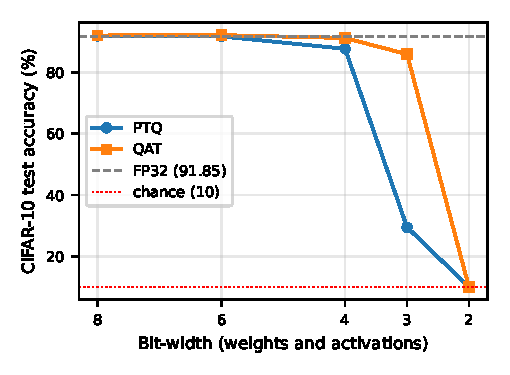
\includegraphics[width=0.92\columnwidth]{bits_vs_acc.pdf}
\caption{Accuracy against bit-width for PTQ and QAT. The dashed line is the float model, the dotted line is chance level.}
\label{fig:bits}
\end{figure}

Three things stand out. First, 8 and 6 bits are as good as float with either method, in line with the paper's finding that 8 and 7 bits behave alike. Second, the value of QAT grows quickly as bits are removed: it is negligible at 8 bits, 3.5 points at 4 bits and over 56 points at 3 bits, where PTQ has almost broken down. Third, the paper's lowest setting is 4 bits (where it saw its largest drops on MobileNet face-attribute models, about 14\% relative for 4/4 bits); our ResNet-18 loses only 0.7\% relative at 4 bits with QAT, which may be because ResNet-18 is larger and CIFAR-10 is easier, but we did not test this. Bit-widths of 3 and 2 are not covered in the paper, so these two rows are our own addition.

\section{Failure Cases and Limitations}
\textbf{2-bit collapse.} Both PTQ and QAT end at exactly 10\%, i.e.\ chance. In QAT the accuracy was 16.7\% after the first epoch and exactly 10.00\% in the next three, which means the network predicts one class for every image. With the range $[1,3]$ the weights have only three levels and the activations four, so very little capacity is left, but we did not diagnose the cause (a lower learning rate, more epochs or per-channel scales might help).

\textbf{3-bit instability.} QAT accuracy went 83.99, 83.40, 83.02, 85.94 over four epochs, so training had not converged; more epochs would probably give a better number.

\textbf{Other limitations.} (i) One seed, no confidence intervals. (ii) QAT gets four epochs more than the float model, so gains at 8 and 6 bits are not evidence for improvement over float. (iii) We did not try MobileNetV2, where the paper expects PTQ to hurt more. (iv) Latency was measured with PyTorch's kernels on a desktop-class CPU, not on a phone. (v) The \texttt{torch.ao.quantization} API used for the int8 benchmark prints a deprecation warning and is scheduled for removal in a later PyTorch release.

\textbf{Differences from the paper.} Dataset and model (CIFAR-10, ResNet-18); batch-norm is folded once before QAT instead of being simulated during training; activation-range EMA uses momentum 0.9 and there is no delayed start of activation quantization (we start from a calibrated PTQ model instead); we quantize the input of every convolution and linear layer, so the identity shortcut and the residual addition of ResNet stay in float while the paper quantizes after the addition; ResNet-18 uses ReLU, not ReLU6; we compute with $(q_1-Z_1)$ directly as in (\ref{eq:int}) and do not use the paper's zero-point optimization; our rescaling shift rounds ties upward, whereas the paper recommends rounding ties away from zero to avoid a bias; QAT is only 4 epochs.

\section{Conclusion}
We rebuilt the affine quantizer, the fake-quantization layer with STE, activation range tracking and the integer-only computation of Jacob et al.\ and tested them on ResNet-18 and CIFAR-10. The main trends of the paper appear at our scale: 8-bit models match float accuracy, the model is about four times smaller, int8 inference is faster, and training with simulated quantization matters when bits are removed. The size of the accuracy drop in the paper was not reproduced, and our experiments are limited by a single seed, short QAT runs and one model.

\begin{thebibliography}{9}
\bibitem{jacob2018} B.~Jacob, S.~Kligys, B.~Chen, M.~Zhu, M.~Tang, A.~Howard, H.~Adam, and D.~Kalenichenko, ``Quantization and training of neural networks for efficient integer-arithmetic-only inference,'' in \emph{Proc.\ IEEE/CVF Conf.\ Computer Vision and Pattern Recognition (CVPR)}, 2018. arXiv:1712.05877.
\bibitem{bengio2013} Y.~Bengio, N.~L\'eonard, and A.~Courville, ``Estimating or propagating gradients through stochastic neurons for conditional computation,'' arXiv:1308.3432, 2013.
\bibitem{he2016} K.~He, X.~Zhang, S.~Ren, and J.~Sun, ``Deep residual learning for image recognition,'' in \emph{Proc.\ CVPR}, 2016.
\bibitem{krizhevsky2009} A.~Krizhevsky, ``Learning multiple layers of features from tiny images,'' Univ.\ of Toronto, Tech.\ Rep., 2009.
\bibitem{paszke2019} A.~Paszke \emph{et al.}, ``PyTorch: An imperative style, high-performance deep learning library,'' in \emph{Advances in Neural Information Processing Systems (NeurIPS)}, 2019.
\end{thebibliography}

\end{document}
